\chapter{Proposed Work}
\label{ch:proposed}

This chapter describes the data, the models and the evaluation protocol.
All settings are the defaults in \texttt{configs/config.py}
(Appendix~\ref{app:config}); each experiment changes exactly one of them.

\section{Dataset and Preprocessing}
\label{sec:dataset}
We use the TB Chest X-ray Database of Rahman et al.~\cite{rahman2020}: 4,200
posterior--anterior radiographs, 3,500 \emph{Normal} and 700
\emph{Tuberculosis}, mostly at $512 \times 512$ pixels. Because the classes
are imbalanced 5:1, a model that always answers ``Normal'' reaches 83.3\%
accuracy, so we report recall, F1 and ROC-AUC alongside accuracy and treat
F1 as the main summary metric.

Each image is converted to grayscale, resized to $64 \times 64$ pixels and
scaled to $[-1, 1]$; the resized images are cached once. No augmentation is
used, so differences between models cannot come from augmentation
randomness. The low resolution is a deliberate compromise that keeps more
than 150 training runs, including 4.3 million simulated circuits for the
quanvolution, feasible on a laptop CPU; we discuss it as a limitation.

The dataset has no official split, so we use a stratified 70/15/15 split
with a fixed seed (Table~\ref{tab:split}). The split seed is separate from
the training seed, so repeating an experiment with seeds 42, 43 and 44
changes only weight initialisation and batch order, and every model is
scored on the same 630 test images. Low-data experiments draw a stratified
2\%, 5\%, 10\% or 25\% of the training split; the validation and test sets
are never reduced.

\begin{table}[htbp]
\centering
\caption{Stratified split of the TB Chest X-ray Database used in all experiments.}
\label{tab:split}
\begin{tabular}{lrrr}
\toprule
Split & Normal & Tuberculosis & Total \\
\midrule
Training   & 2,450 & 490 & 2,940 \\
Validation &   525 & 105 &   630 \\
Test       &   525 & 105 &   630 \\
\bottomrule
\end{tabular}
\end{table}

\section{Models}
\label{sec:models_overview}
Every model maps an image through a \emph{backbone} to a 32-dimensional
embedding and through a \emph{head} to the probability of TB. The hybrids
differ from the classical baseline in one place only: the head (\cq) or an
input transform in front of the backbone (\qc), as shown in
Figure~\ref{fig:architectures}.

\begin{figure}[htbp]
  \centering
  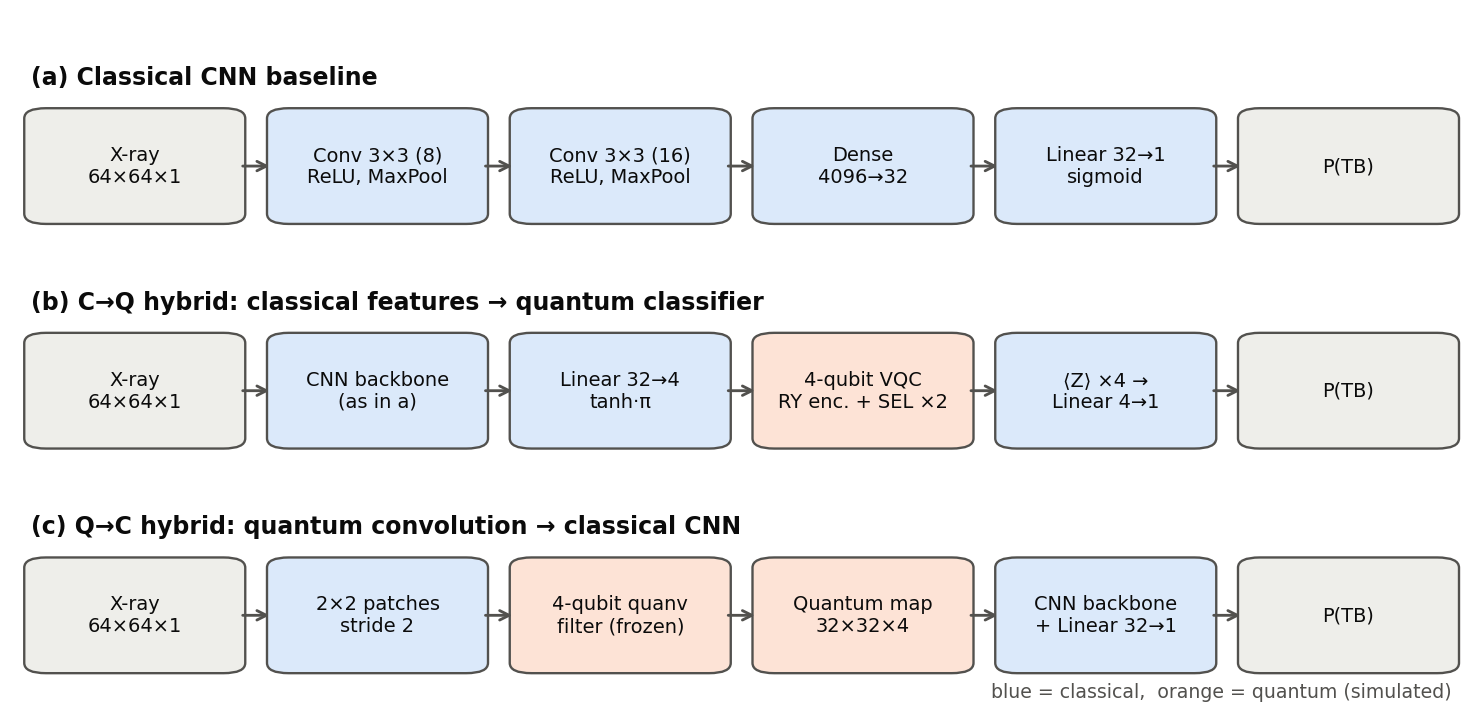
\includegraphics[width=\linewidth]{architectures.png}
  \caption{The three architectures: (a) classical CNN baseline,
  (b) classical-to-quantum hybrid, (c) quantum-to-classical hybrid. Blue
  blocks are classical, orange blocks are quantum.}
  \label{fig:architectures}
\end{figure}

\subsection{Classical CNN Baseline}
\label{sec:baseline}
The backbone has two blocks of $3 \times 3$ convolution (8 and 16 filters,
padding 1), ReLU~\cite{nair2010} and $2 \times 2$ max pooling, followed by
a dense projection of the $16 \times 16 \times 16$ feature map to 32 values
(131,104 parameters). The classical head is a linear layer with a sigmoid
(33 parameters). The model has 132,385 parameters in total; it is
deliberately small, so that the quantum component is not hidden behind a
very powerful classical network.

\subsection{Classical-to-Quantum (\cq) Hybrid}
\label{sec:cq}
The \cq{} hybrid replaces the linear head with a ``dressed'' variational
quantum classifier~\cite{mari2020}. A linear layer compresses the embedding
to $n = 4$ values $\mathbf{u}$, which are scaled to
$\mathbf{x} = \pi\tanh(\mathbf{u}) \in (-\pi, \pi)$ so that no two feature
values map to the same rotation, and encoded as
$\bigotimes_k R_Y(x_k)\ket{0}$. Two StronglyEntanglingLayers follow; each
applies $\mathrm{Rot}(\phi,\theta,\omega)$ to every qubit and a ring of
CNOTs of range 1 (first layer) and 2 (second layer), giving a weight tensor
of shape $(L, n, 3)$, i.e.\ 24 parameters. The four expectation values
$\expval{Z_k}$ (Eq.~\ref{eq:expz}) pass through a linear layer and a sigmoid
(Figure~\ref{fig:circuit_cq}). The head has 161 parameters and the whole
model 132,513, only 128 more than the baseline. The circuit is simulated with
PennyLane's \texttt{default.qubit} simulator inside a
\texttt{qml.qnn.TorchLayer}, so it trains like any PyTorch layer.

\begin{figure}[htbp]
  \centering
  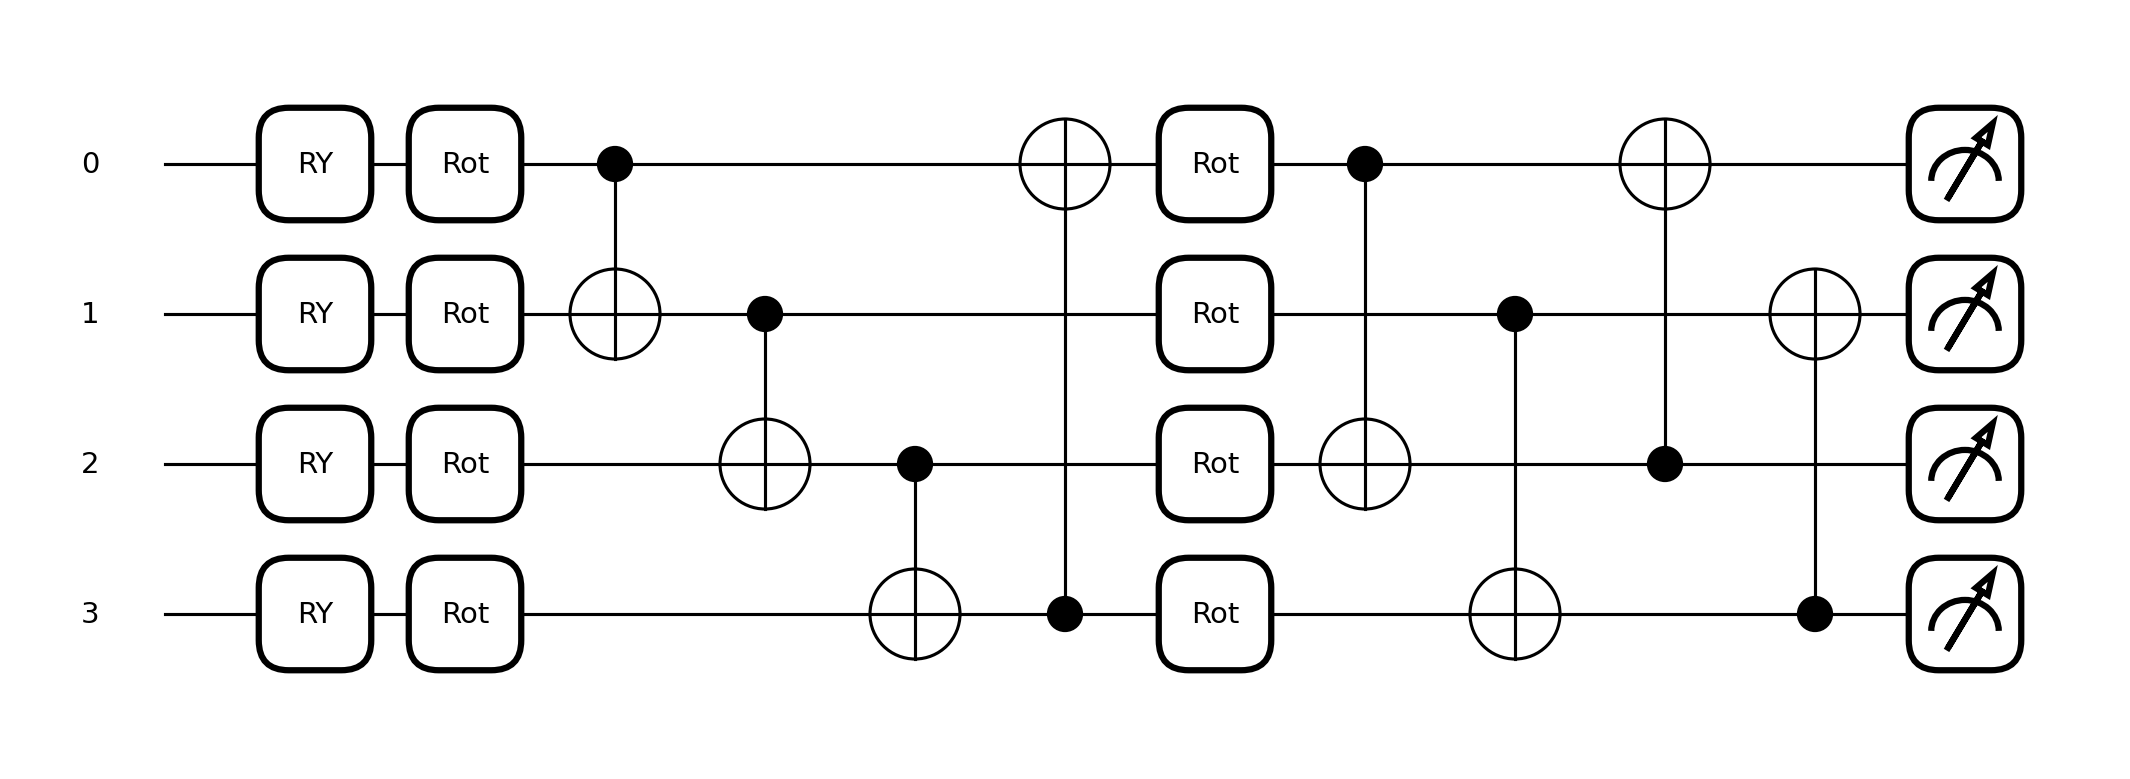
\includegraphics[width=0.85\linewidth]{circuit_cq_strong.png}
  \caption{Quantum circuit of the \cq{} head (4 qubits, depth 2): $R_Y$
  encoding, two StronglyEntanglingLayers, and measurement of $\expval{Z}$ on
  every qubit.}
  \label{fig:circuit_cq}
\end{figure}

For the ablation the head can use depth $L \in \{1,2,3,4\}$, $n \in
\{2,4,6,8\}$ qubits, amplitude encoding (the compression layer then outputs
$2^n$ values), BasicEntanglerLayers (one $R_X$ per qubit and a
nearest-neighbour CNOT ring), or no entanglement (the same rotations without
CNOTs, equivalent to four independent one-qubit models).

\subsection{Quantum-to-Classical (\qc) Hybrid}
\label{sec:qc}
The \qc{} hybrid places a quantum circuit at the start of the network as a
convolution filter~\cite{henderson2020}. The image is divided into 1,024
non-overlapping $2 \times 2$ patches; each pixel $p_k \in [0,1]$ is encoded
as $R_Y(\pi p_k)$, a fixed random circuit (one PennyLane \texttt{RandomLayers}
layer, seed 0, Figure~\ref{fig:circuit_quanv}) is applied, and the four
$\expval{Z_k}$ become four output channels. The resulting $4 \times 32
\times 32$ quantum feature map (Figure~\ref{fig:quanvmaps}) is processed by
the same CNN with four input channels. Because the input is half the size,
the model has only 34,297 parameters. As in the original method the filter
is random and frozen, so the transform is computed once for all 4,200 images
(4.3 million four-qubit circuits) and cached.

\begin{figure}[htbp]
  \centering
  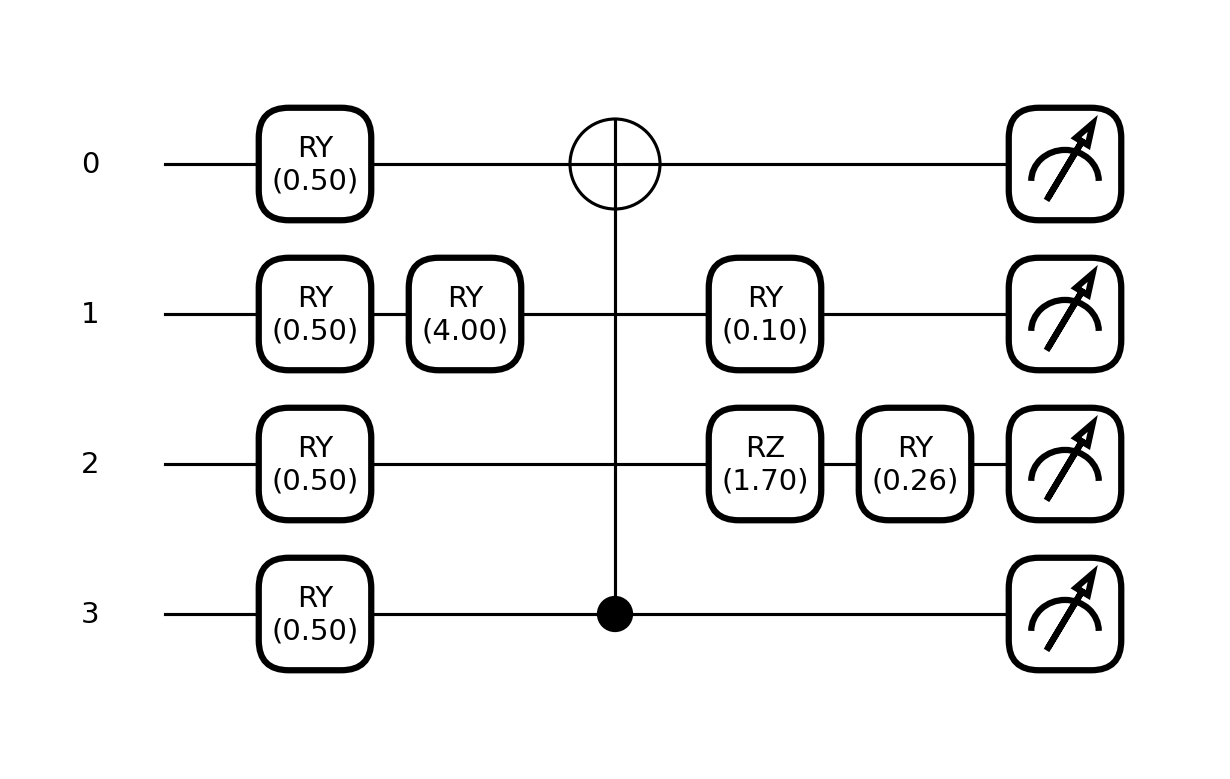
\includegraphics[width=0.5\linewidth]{circuit_quanv.png}
  \caption{The quanvolution filter for one $2\times2$ patch (encoding angles
  set to 0.5 for display). Its gates are drawn once from a fixed seed and not
  trained.}
  \label{fig:circuit_quanv}
\end{figure}

\begin{figure}[htbp]
  \centering
  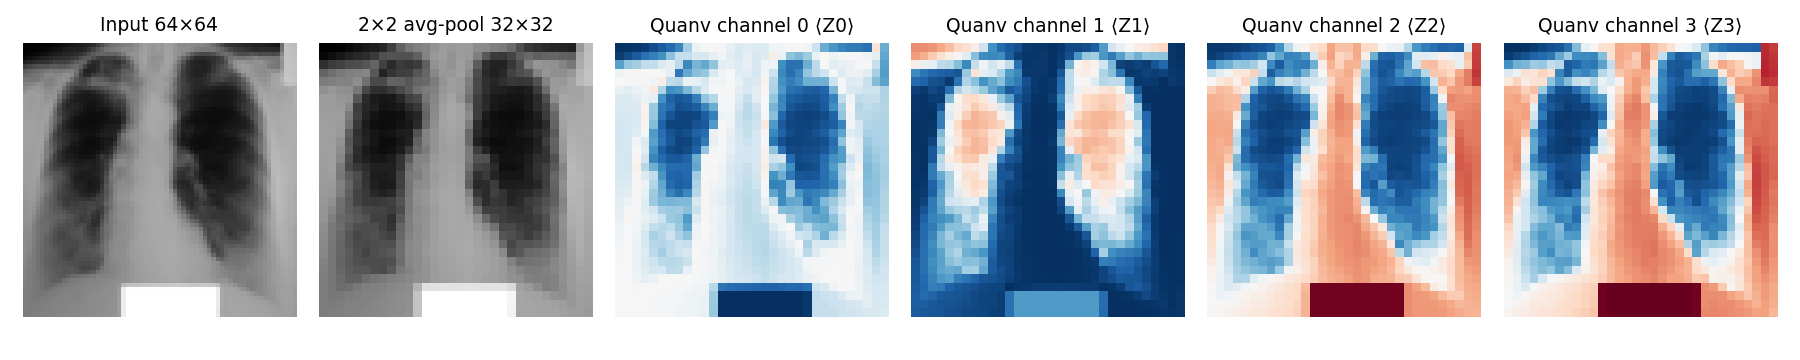
\includegraphics[width=\linewidth]{quanv_feature_maps.png}
  \caption{A TB radiograph at $64\times64$, its $2\times2$ average-pooled
  version, and the four channels of its quanvolution feature map. The
  rectangle at the bottom is a marker burned into the image, not anatomy.}
  \label{fig:quanvmaps}
\end{figure}

\subsection{Classical Control Models}
\label{sec:controls}
A hybrid that beats a baseline does not prove that its circuit is useful,
because it also differs in structure. Each hybrid is therefore paired with
classical models that differ from it only in the quantum component
(Table~\ref{tab:controls}). The matched head mirrors the quantum head step
for step, so any difference can only come from \emph{what} the four-to-four
transformation computes. The three \qc{} controls separate three
explanations: any fixed non-linear patch map, the downsampling itself, and
a patch filter that is allowed to learn.

\begin{table}[htbp]
\centering
\footnotesize
\caption{Models in the main study and what each one controls for.}
\label{tab:controls}
\begin{tabular}{p{4.2cm}rp{7.2cm}}
\toprule
Model & Params & Purpose \\
\midrule
Classical CNN & 132,385 & Baseline. \\
CNN + matched classical head & 132,509 & Control for \cq: the circuit is
replaced by a classical $\mathrm{Linear}(4,4)$ and $\tanh$ (157 head
parameters versus 161). \\
\cq{} hybrid & 132,513 & CNN + variational quantum head. \\
\midrule
\qc{} hybrid & 34,297 & Quanvolution + CNN. \\
Random patch + CNN & 34,297 & Control for \qc: fixed random classical map
$\tanh(W\pi\mathbf{p} + \mathbf{b})$ with the same input and output. \\
Avg-pool + CNN & 34,081 & Control for \qc: plain $2\times2$ average pooling. \\
Learned $2\times2$ conv + CNN & 34,317 & Control for \qc: trainable
$2\times2$, stride-2 convolution with four channels and $\tanh$. \\
\bottomrule
\end{tabular}
\end{table}

\subsection{Transfer Learning with ResNet18}
\label{sec:resnet}
To test the findings with a strong backbone, the small CNN is replaced by an
ImageNet-pretrained ResNet18~\cite{he2016}. The grayscale channel is
repeated three times, the ImageNet classifier is replaced by a linear layer
to the same 32-dimensional embedding, so either head can be attached, and
the pretrained layers are fine-tuned with a ten times smaller learning rate
($10^{-4}$). The resulting models have about 11.19 million parameters.

\section{Training and Evaluation Protocol}
\label{sec:training}
All models are trained identically: binary cross-entropy
(Eq.~\ref{eq:bce}), Adam~\cite{kingma2015} with learning rate $10^{-3}$,
batch size 32 and 15 epochs on a CPU, with no per-model tuning. In the main
study every run keeps the weights of the epoch with the lowest validation
loss, and runs on 2--10\% of the data train for 40 epochs, since 15 epochs
on 58 images are only about 30 gradient steps. Quantum gradients are
computed by backpropagation through the simulator; on hardware the
parameter-shift rule (Eq.~\ref{eq:pshift}) would be used, and we verify that
the two agree.

\label{sec:eval}
An image is predicted as TB when its probability is at least 0.5. With TB as
the positive class we report
\begin{align}
\mathrm{Accuracy} &= \frac{TP + TN}{TP + TN + FP + FN}, &
\mathrm{Recall} &= \frac{TP}{TP + FN}, \\
F_1 &= \frac{2\cdot\mathrm{Precision}\cdot\mathrm{Recall}}{\mathrm{Precision}+\mathrm{Recall}}, &
\mathrm{Precision} &= \frac{TP}{TP + FP},
\end{align}
and the ROC-AUC, the probability that
a random TB image is scored above a random normal image~\cite{fawcett2006}.
Recall matters most clinically, since a missed TB case is more harmful than
a false alarm. Multi-seed experiments report mean $\pm$ standard deviation
over seeds 42, 43 and 44, and any ``best'' configuration is chosen on
validation F1, never on the test set.

Because all models are scored on the same test images, two models are
compared image by image with McNemar's exact test~\cite{mcnemar1947}. If $b$
images are classified correctly by model A only and $c$ by model B only, then
under the null hypothesis of equal error rates
$b \sim \mathrm{Binomial}(b + c, \tfrac{1}{2})$. The test is run separately
for each seed, and $p < 0.05$ is treated as significant.

\label{sec:qa_protocol}
The circuits are also characterised directly: expressibility and entangling
capability of the trainable block (three entanglement patterns, depths 1--4,
5,000 random parameter pairs); the variance over 500 random initialisations
of the gradient of a local cost $\expval{Z_0}$ and a global cost
$\expval{Z^{\otimes n}}$ for 2 to 10 qubits at depths 2 and 10; the trained
\cq{} model (seed 42) re-evaluated with 10 to 10,000 measurement shots and
with depolarising noise (Eq.~\ref{eq:depol}) after every layer for $p$ up to
0.2, with its weights fixed; and a comparison of parameter-shift and
backpropagation gradients of the trained circuit.
